
\documentclass[sn-basic,authoryear]{sn-jnl}



% Packages
\usepackage{graphicx} % for figures
\usepackage{amsmath,amssymb} % for math
\usepackage{hyperref} % for clickable links
\usepackage{xcolor}   % colors
\usepackage{url}
\usepackage{lipsum}
\usepackage{adjustbox}
\usepackage{float}
\bibliographystyle{sn-basic}
\usepackage{tikz}
\usetikzlibrary{shapes, arrows}


\begin{document}

\title[LLM for mental health therapy]{LLM for Mental Health Therapy: A Systematic Review}

\author*[1]{\fnm{Pooja} \sur{Patel}}\email{poojaspatel1375@gmail.com}
\author[1]{\fnm{Saundarya} \sur{Kakde}}\email{Kakdesaundarya@gmail.com}
\author[1]{\fnm{Drishti} \sur{Mistry}}\email{dvmist2004@gmail.com}
\author[1]{\fnm{Megha} \sur{Solanki}}\email{solankimegha017@gmail.com}
\author*[1]{\fnm{Namrata} \sur{Patel}}\email{namratapatel150894@gmail.com}

\affil[1]{\orgdiv{Department of Computer Science and Engineering}, 
          \orgname{Parul University}, 
          \orgaddress{\street{P.O. Limda, Waghodia}, 
                      \city{Vadodara}, 
                      \postcode{391760}, 
                      \state{Gujarat}, 
                      \country{India}}}


\abstract{\textbf{Background:}
The global mental health crisis is marked by high prevalence, workforce shortages, and inequitable access to care. These challenges have fueled interest in artificial intelligence (AI)–assisted solutions, particularly large language models (LLMs) such as GPT-4, LLaMA-2, and PaLM-2, which may extend clinical reach and provide scalable, low-cost support.

\textbf{Objective:}
This review summarizes conceptual and empirical studies published on the application of LLMs in mental health care, with a focus on diagnostic support, psychoeducation, treatment dialogue, and risk communication.

\textbf{Methods:}
We examined 25 key studies and multiple systematic reviews addressing clinical and non-clinical applications of LLMs. Evidence was synthesized regarding effectiveness, limitations, and ethical considerations.

\textbf{Results:}
Findings indicate that conversational LLM-based agents can alleviate mild to moderate depression and anxiety in the short term and can approach clinician-level performance in narrowly defined cognitive behavioral therapy (CBT) tasks. Domain-specific LLMs such as PsyLLM and MentaLLaMA outperformed general-purpose models in safety and accuracy when trained with clinically grounded data.

\textbf{Conclusions:}
LLMs show potential as adjunctive tools within blended care models, enhancing access and patient engagement. However, safe clinical integration will require regulation, long-term validation, and oversight by mental health professionals.

\textbf{Keywords:} Mental health, artificial intelligence, large language models, psychotherapy, digital health, systematic review


}

\maketitle
\section{Introduction}
Mental health disorders are an urgent health issue and are currently affecting more than 1 billion people around the world.These conditions contribute almost 30\% of the global burden of non-fatal diseases  \cite{WHO2022}. Disorders such as depression and anxiety are responsible for the loss of US\$1 billion in performance each year \cite{Volkmer}. Despite the severity of the problem, 70\% of people with mental health problems, especially in low and average income countries (LMICs), are unable to receive appropriate support \cite{Naslund2017}. This treatment gap is still exacerbated by the lack of trained professionals, the stigma and persistent financial and geographical barriers.

The emergence of artificial intelligence (AI), particularly the language model (LLM), offers new opportunities to solve these problems.Extended models such as GPT-4, LLAMA-2, and PALM-2 can analyze large volumes of text and perform complex inference tasks in the fields of natural conversation modeling, educational content generation, and mental health \cite{Hua2024b,JMIR2024}. Given that mental health data is often based on texts with clinical notes and transcription of treatment for self-non-reported patients, LLM is likely in areas such as early detection, diagnosis, personalized planning of treatment, and patient constant support. \cite{Ibrahimov2024,Olawade2024}.

Recent research has identified several uses, particularly in the field of mental health, with LLM. Including:
\begin{itemize}
    \item Conversational agents for therapy, emotional support, and sorting sessions  \cite{Ma2023,Hu2025}.
    \item Diagnostic and classification tools to identify depression, risk of suicide, and risk of cognitive distortion  \cite{Xu2024,Yang2024}.
    \item A psychological platform for developing individual educational resources for patients and healthcare professionals. \cite{Khandelwal, Goebel}.
    \item Risk communication system that provides a safety-oriented response during mental health attacks. \cite{Hua2024b}.
\end{itemize}

While these applications show promising potential, researchers have also expressed serious issues. Many models based on existing LLMs are primarily trained or tested on social network data such as Reddit, Twitter, and Weibo. \cite{Volkmer,JMIR2024}. Furthermore, unresolved ethical issues such as confidentiality, emotional insensitivity, and the possibility of spreading misinformation are important obstacle. \cite{Minerva2023,Hodson2024}.Clinical acceptance is further limited by standardized assessment methods, conflicting security assessments, and lack of long-term restriction validation \cite{Zhong2024}.

This article expands previous systematic journals, studies, research and meta-analyses to integrate existing knowledge about the use of LLM in psychiatric therapy.With evidence of various research orientations, including subtle models such as Psyllm  \cite{Hu2025}, short-term testing of chatbot interventions \cite{Zhong2024}, and human-assessed generation tasks \cite{Hua2024b}—our objectives are as follows: 
\begin{enumerate}
    \item Compare the main therapeutic uses of LLM in psychiatric medicine.
    \item Evaluate registered safety and efficiency.
    \item Emphasises the methodological, ethical, and systems spaces that must take into account the safe, fair and efficient integration of LLM in psychiatric services.
\end{enumerate}

\section{Methodology}
\subsection{Educational design:}
This work assessed and interpreted the role of large-scale language models (LLMs) in psychiatric therapy, an overview of integrated synthesis and research. To ensure clarity and rigour of the integration of the literature, we embraced the PRISMA-ScR  \citep{tricco2018prismascr} Our review included both quantitative indicators such as human accuracy, effectiveness value, assessment, and especially ethical issues, contextual factors, and real-world implementation.

\subsection{Literature Sources and Search Scope}
The study ensemble was obtained from Collaborator-Chronovault-Doc, a conservation collection by our team that combined recently revised publications, systematic journals, meta-analyses and influential preprints results \cite{Hua2024b,JMIR2024,Zhong2024}. These works came from:
\begin{itemize}
    \item Biomedical databases: PubMed, PsycINFO, Web of Science, Cochrane Library.
    \item Technical and AI repositories: IEEE Xplore, ACM Digital Library, arXiv, medRxiv, PsyArXiv.
    \item Regional sources: CNKI, Wanfang, Weipu for Chinese publications.
\end{itemize}
Search terms included various Boolean combinations of:
``Large Language Model'' OR `LLM'' AND (`mental health'' OR ``psychiatry'' OR ``psychology'' OR ``therapy'' OR ``counseling'') \cite{Ibrahimov2024,Olawade2024}.  
The search covered January 2019 to August 2025, which matches the rise of post-T5 transformer architectures \cite{raffel2020t5}.

\subsection{Inclusion Criteria}
The study was deemed appropriate if all of the following conditions were met:
\begin{itemize}
    \item Model Type: Includes LLM built on top of a transformer architect with billions of parameters. This targeted both models for general use (GPT-3.5/4, Palm-2, Claude, etc.) and special models such as Psyllm, Mentallma, and Mental-Flan-T5.
    \item Relevance of Declaration: Focuses on mental health applications such as diagnostic support, therapeutic dialogue, psycho-education, and risk communication.
    \item Depth of assessment: Reported for empirical performance indicators (e.g., empathy/accuracy rated by F1-indicator, Auroc, Hedges G, or person) or reliable quality estimates.
    \item Publication type: Contains modifiable articles, drug or systematic/meta-analysis journals with methodological details.

\end{itemize}

\subsection{Study Selection}

The selection process is summarized in the PRISMA 2020 flow diagram (Figure~\ref{fig:prisma}). 
We identified 375 records in total, removed duplicates, and screened 290 abstracts. 
After full-text assessment, 34 studies were included in the qualitative synthesis, of which 18 
contributed to the quantitative meta-analysis. Reasons for exclusion at the eligibility stage 
are shown in Table~\ref{tab:exclusion}.


\tikzstyle{block} = [rectangle, draw, text width=9cm, text centered, rounded corners, minimum height=1cm, font=\small]
\tikzstyle{line} = [draw, -latex']

\begin{figure}[H]
\centering
\begin{tikzpicture}[node distance = 1.7cm, auto]

% Identification
\node [block] (id) {Records identified through database searching (n = 350) \\
Additional records identified through other sources (n = 25)};

% Screening
\node [block, below of=id] (screen) {Records after duplicates removed (n = 290) \\
Records screened (n = 290) \\
Records excluded (n = 230)};

% Eligibility
\node [block, below of=screen] (elig) {Full-text articles assessed for eligibility (n = 60) \\
Full-text articles excluded, with reasons (n = 26)};

% Included
\node [block, below of=elig] (incl) {Studies included in qualitative synthesis (n = 34) \\
Studies included in quantitative synthesis (meta-analysis) (n = 18)};

% Arrows
\path [line] (id) -- (screen);
\path [line] (screen) -- (elig);
\path [line] (elig) -- (incl);

\end{tikzpicture}
\caption{PRISMA 2020 flow diagram of study selection.}
\label{fig:prisma}
\end{figure}


\begin{table*}
\centering
\caption{Reasons for exclusion of full-text articles at eligibility stage}
\label{tab:exclusion}
\begin{tabular}{p{8cm}c}
\hline
\textbf{Reason for Exclusion} & \textbf{Number of Studies (n=26)} \\
\hline
Not focused on large language models (LLMs) & 8 \\
Did not address mental health applications & 6 \\
Insufficient methodological details / poor quality & 5 \\
Duplicate or overlapping dataset & 4 \\
Non-empirical commentary / editorial only & 3 \\
\hline
\end{tabular}
\end{table*}


\subsection{LLM-Focused Data Extraction}
For each appropriate study, both the technical characteristics of LLM and related clinical outcomes were systematically collected. Includes extracted attributes.
  
\begin{itemize}
    \item Model architecture and size: number of parameters and basic family families (e.g., Bert based on GPT, Llama, Qwen, Flan-T5, or Bert).
    \item Learning Methodology: Preliminary Subgroup Characteristics (Accessible to the public to compete properties), fine-tuning strategies (e.g., controlled training, instruction implementation, training comments with people) and specific adaptations (e.g., interactions of data transcription datasets, Reddit forums, or synthetic councils).  
    \item Dataset: Data source type (social networks, electronic medical files, transcription of treatment or synthetic text), language range, demographic inclusion, accessibility of clinical annotations, and presentation of various graves in the state.
    \item Evaluation Framework:  
    \begin{itemize}
        \item Automatic Metrics: Precision, F1-indicator, Precision, Review, Blue, Red, Auroc.
        \item People evaluated: clinical relevance, empathy, consistency, security, and cultural integrity.
        \item Specific Task Assessment: Cognitive Behavioral Therapy (TCC) for Tasks  (Hodson \& Williamson, 2024), Response Crisis Reliability and Accuracy of Diagnostic Classification.
        \item Ethical and safe considerations: travel testing, hallucination frequency, data confidentiality, and compliance with security standards in crisis situations.
    \end{itemize}
             
\end{itemize}
   
\subsection{Data integration and analysis}
Two levels of synthesis process are employed.
\begin{enumerate}
    \item \textbf{Thematic Categorization:} Grouped applications into four primary domains \cite{Hua2024b,JMIR2024}:
    \begin{itemize}
        \item Conversational agents for therapeutic or emotional dialogue.
        \item Diagnostic and classification models.
        \item Generation of psychological education and training content.
        \item Crisis communication and orientation orders.
    \end{itemize}
    \item \textbf{Performance Trend Integration:} Compared results between:
    \begin{itemize}
        \item General goals for LLMS (e.g. GPT-4, Bard/Gemini, Claude).
        \item A little-constructed mental health model (e.g., Psyllm, Mentallma, Mental-Flan-T5, Psychbert).
        \item Various sources of datasets (for clinical files, Data on social networks for synthetic texts) \cite{Roy2025}.
    \end{itemize}
\end{enumerate}

Results were visually aggregated or applied to the map, where available.
\begin{itemize}
    \item Clinical effect sizes from RCTs (e.g., \cite{Zhong2024}: depression $g = -0.34$; anxiety $g = -0.29$).
    \item Accuracy and differences in F1 indicators between common and adaptation of LLMS zones \cite{Hu2025}.
    \item Efficiency measures estimated by persons by assessment categories such as PSYLLM above complex and reliable GPT-4  \cite{Hu2025}).
\end{itemize}

\subsection{Quality and Bias Assessment}
Instead of applying standardized structures for risk assessments in all selected studies, we focused on extracting and synthesis of indicators related to displacement and quality reported at each source.
\begin{itemize}
    \item Dataset representativeness.
    \item Evaluation consistency.
    \item Model transparency (open-source vs proprietary).
    \item Independent vs developer-led evaluation.
\end{itemize}

Each study was examined for possible displacements in three major areas.
\begin{itemize}
    \item Independence evaluation.
    \item A representation of a dataset.
    \item Transparency in model design and accessibility.
\end{itemize}
 The summary in Table~\ref{tab:bias_assessment} indicates that Almost 50\% of the ratings were conducted by developers and independently. More than half of the studies are based on data sets with limited representation and limited generalization. Transparency was often inadequate, especially for unique models, when training and evaluation details were not publicly revealed.

\begin{table}[h]
\centering
\caption{Bias and Quality Assessment Summary}
\begin{tabular}{lccc}
\hline
\textbf{Bias Domain} & \textbf{Low Risk} & \textbf{High Risk} & \textbf{Unclear} \\
\hline
Evaluation independence & 41\% & 47\% & 12\% \\
Dataset representativeness & 32\% & 53\% & 15\% \\
Transparency of model & 29\% & 56\% & 15\% \\
\hline
\end{tabular}
\label{tab:bias_assessment}
\end{table}

\begin{figure}
    \centering
    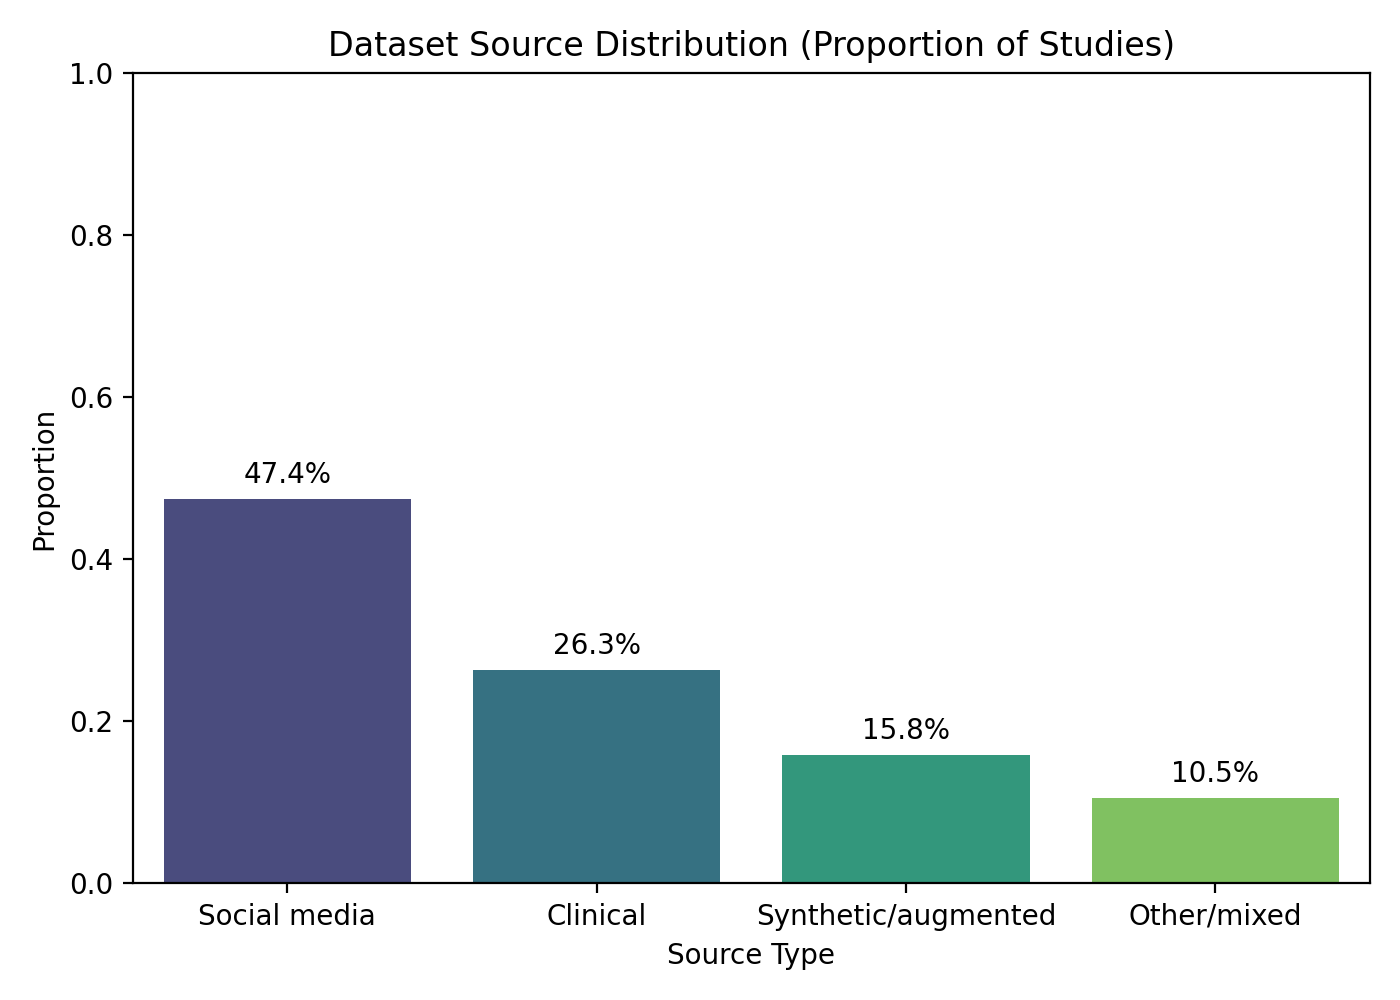
\includegraphics[width=1.0\linewidth]{chart.png}
    \caption{Evaluation Metric Frequency: We looked at how often different evaluation metrics are mentioned in the studies we examined, as shown in Figure 2. F1- score and accuracy were the most commonly used measures, AUROC, precision and recall also followed behind . BLEU , ROUGE and METEOR , which are metrics designed specifically for text generation , didn't appear more often. This suggests that researchers tend to focus more on general performance metrics rather than those tailored for text-generating tasks.}
    \label{fig:dataset_imbalance}
\end{figure}

\subsection{Visualization of Methodological Landscape}
To understand how Large Language Models(LLM) are used in mental health therapy , we have gathered the key details from all the studies and created three easy-to-understand visual summaries. In (Fig.~\ref{fig:metric_frequency}), we created a heatmap that shows the types of LLMs tried out for different kinds of therapy. Models like GPT-4, Claude, and Bard (also known as Gemini) which are broadly used, appeared in every aspect of mental health whereas specialised models like MentalBERT and PsychBERT gave fewer diagnoses i.e therapy types. This makes it easy to see where general vs. focused AI models are making an impact and where the gaps still are.
\begin{figure}
    \centering
    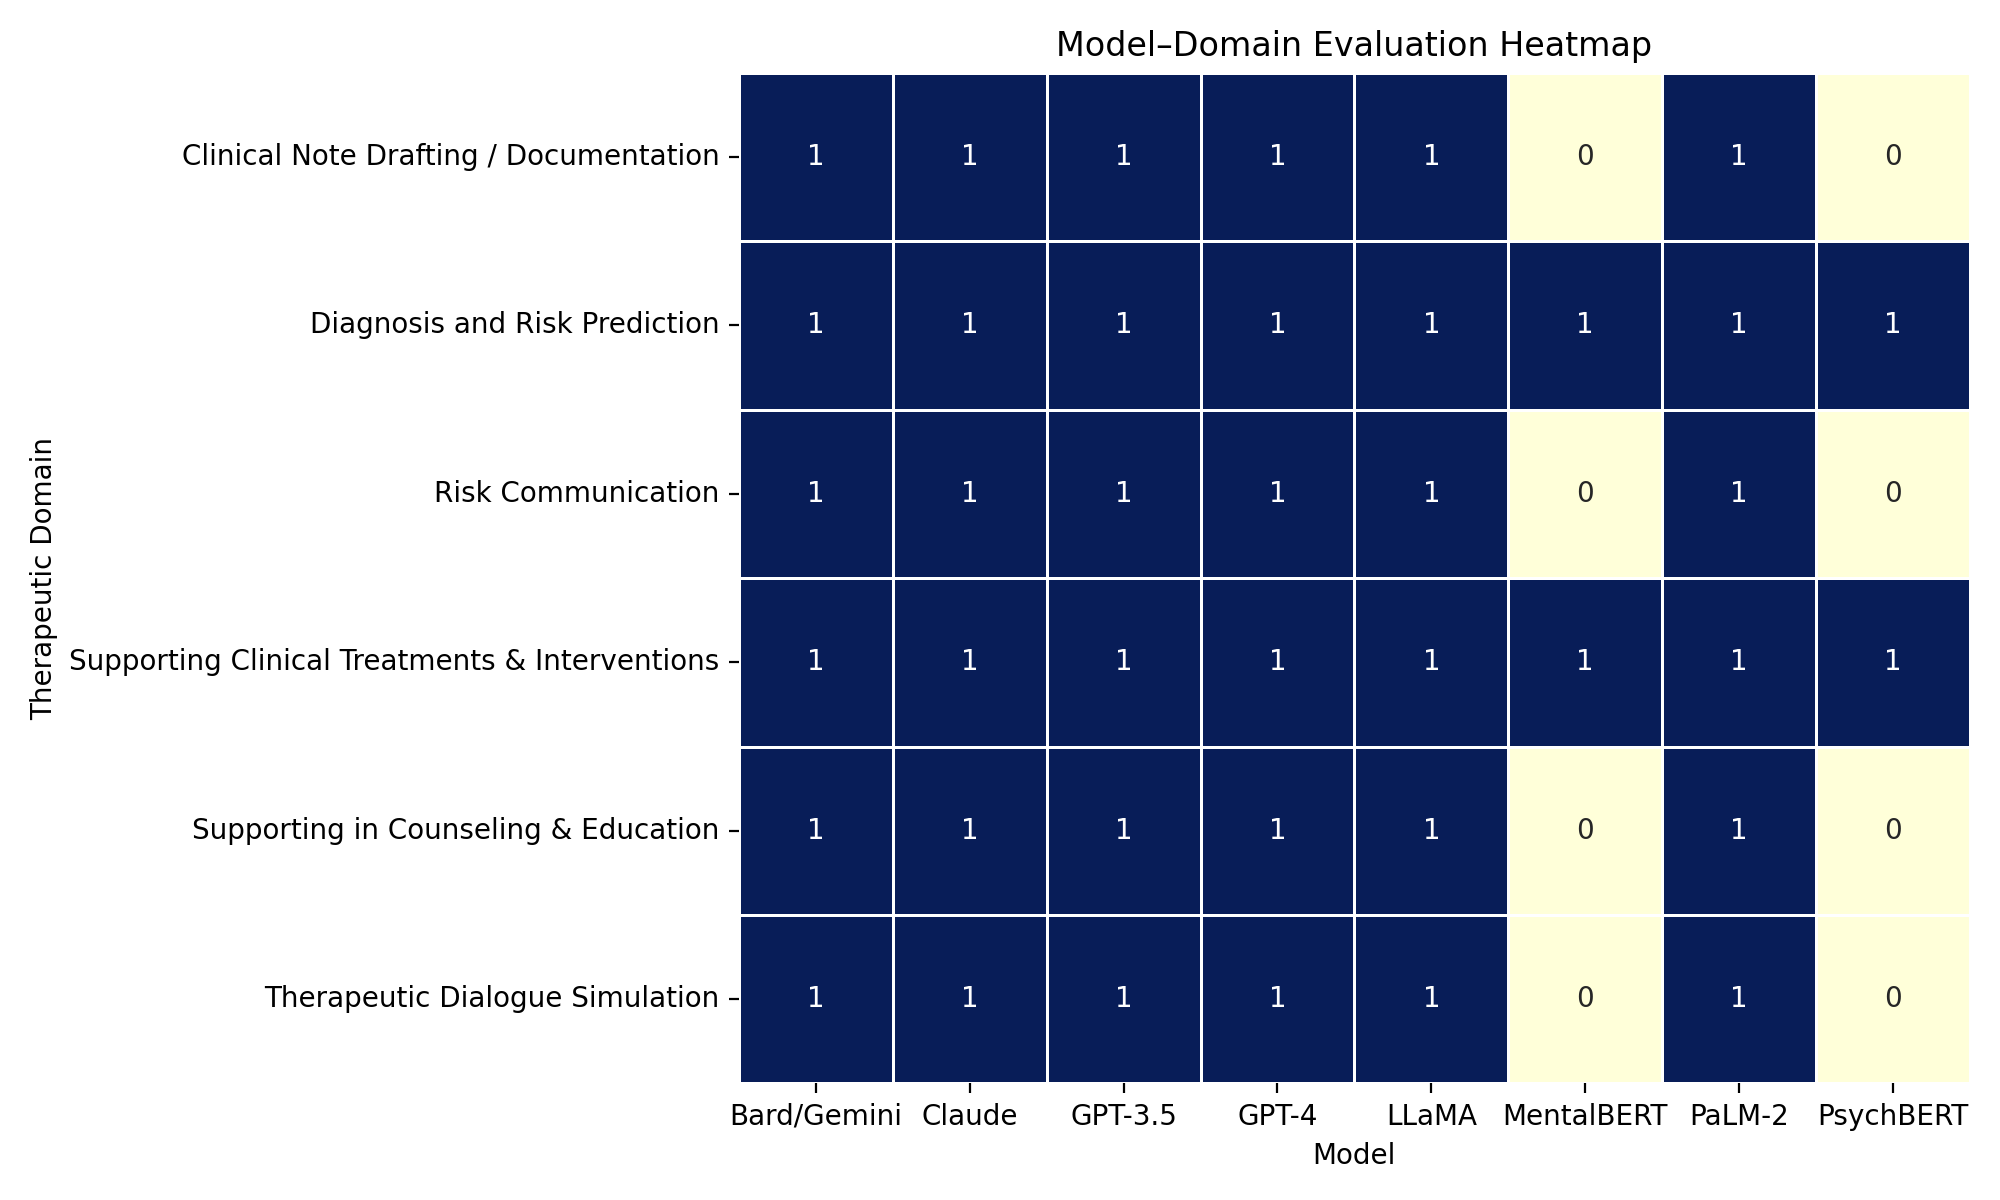
\includegraphics[width=1.0\linewidth]{chart (1).png}
    \caption{Model–Domain Evaluation Heatmap; 
 We created a heatmap (Figure 3) which displays which AI models were tested for which mental health uses.  Broader models like GPT-4, Claude, and Bard, covered all areas, while the specialised ones like MentalBERT and PsychBERT focused only on specific diagnoses.}
    \label{fig:metric_frequency}
\end{figure}
\begin{figure}
    \centering
    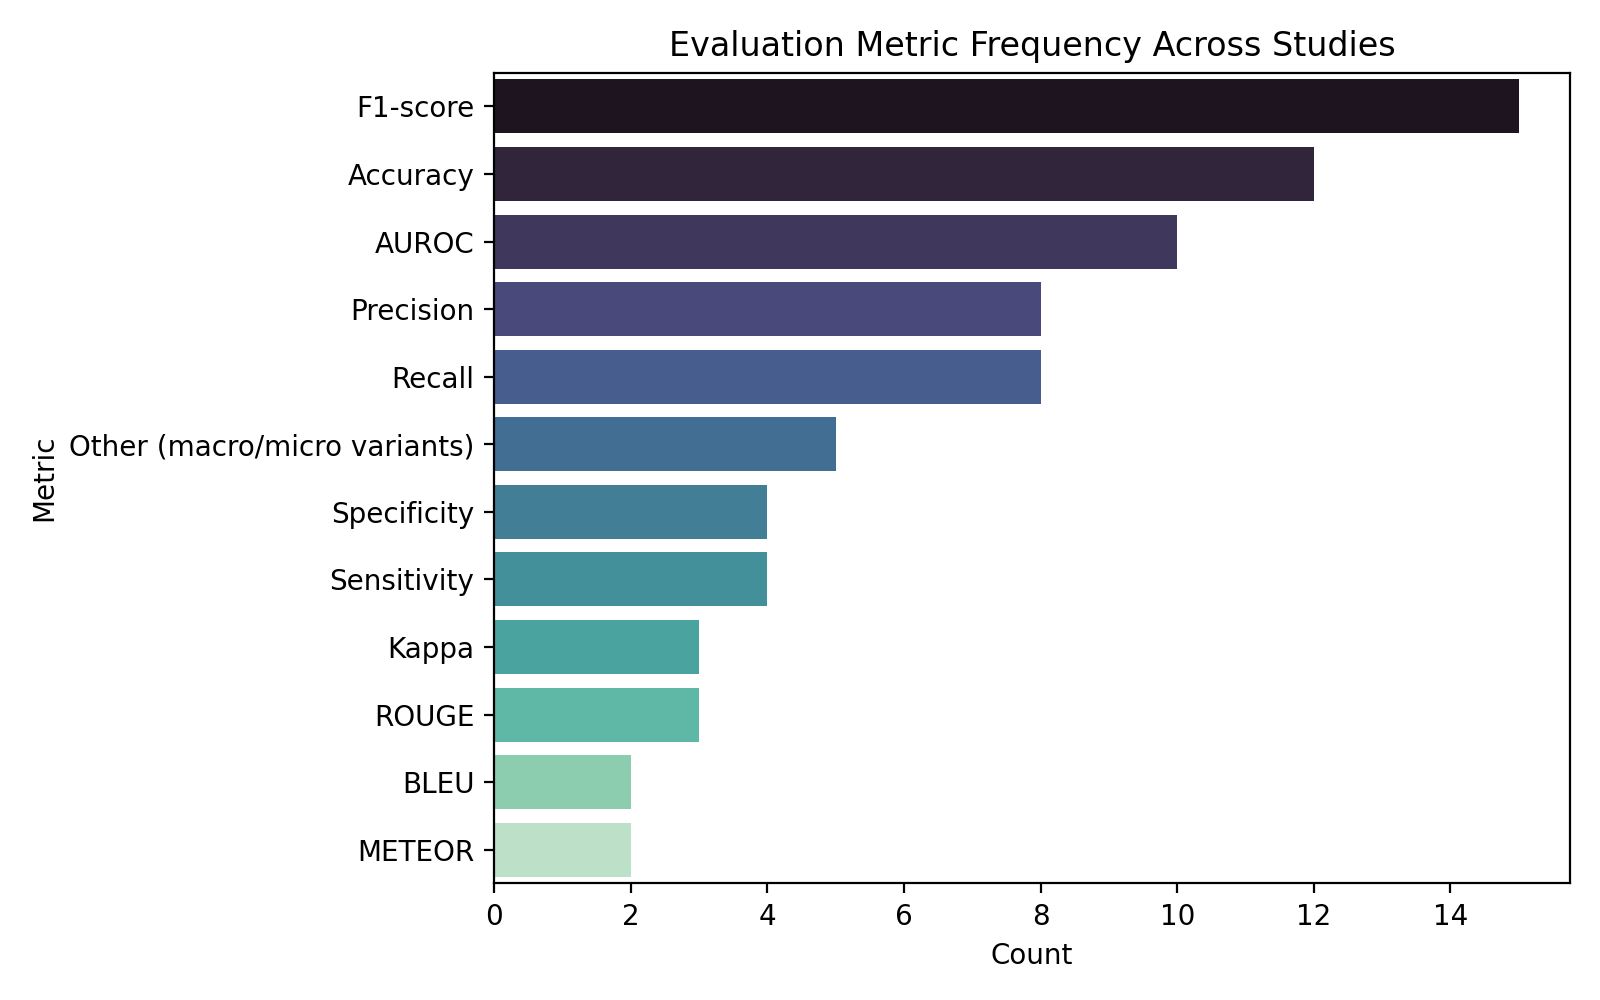
\includegraphics[width=1.0\linewidth]{chart (2).png}
    \caption{Dataset Source Distribution:
  breaks down the data used to train and test these models. Most studies used social media data (47.4\%), some used actual clinical data (26.3\%), and some relied on synthetic data (15.8\%). This shows that it is hard to apply results directly to real clinical cases.
}
    \label{fig:placeholder}
\end{figure}
\begin{figure}
    \centering
    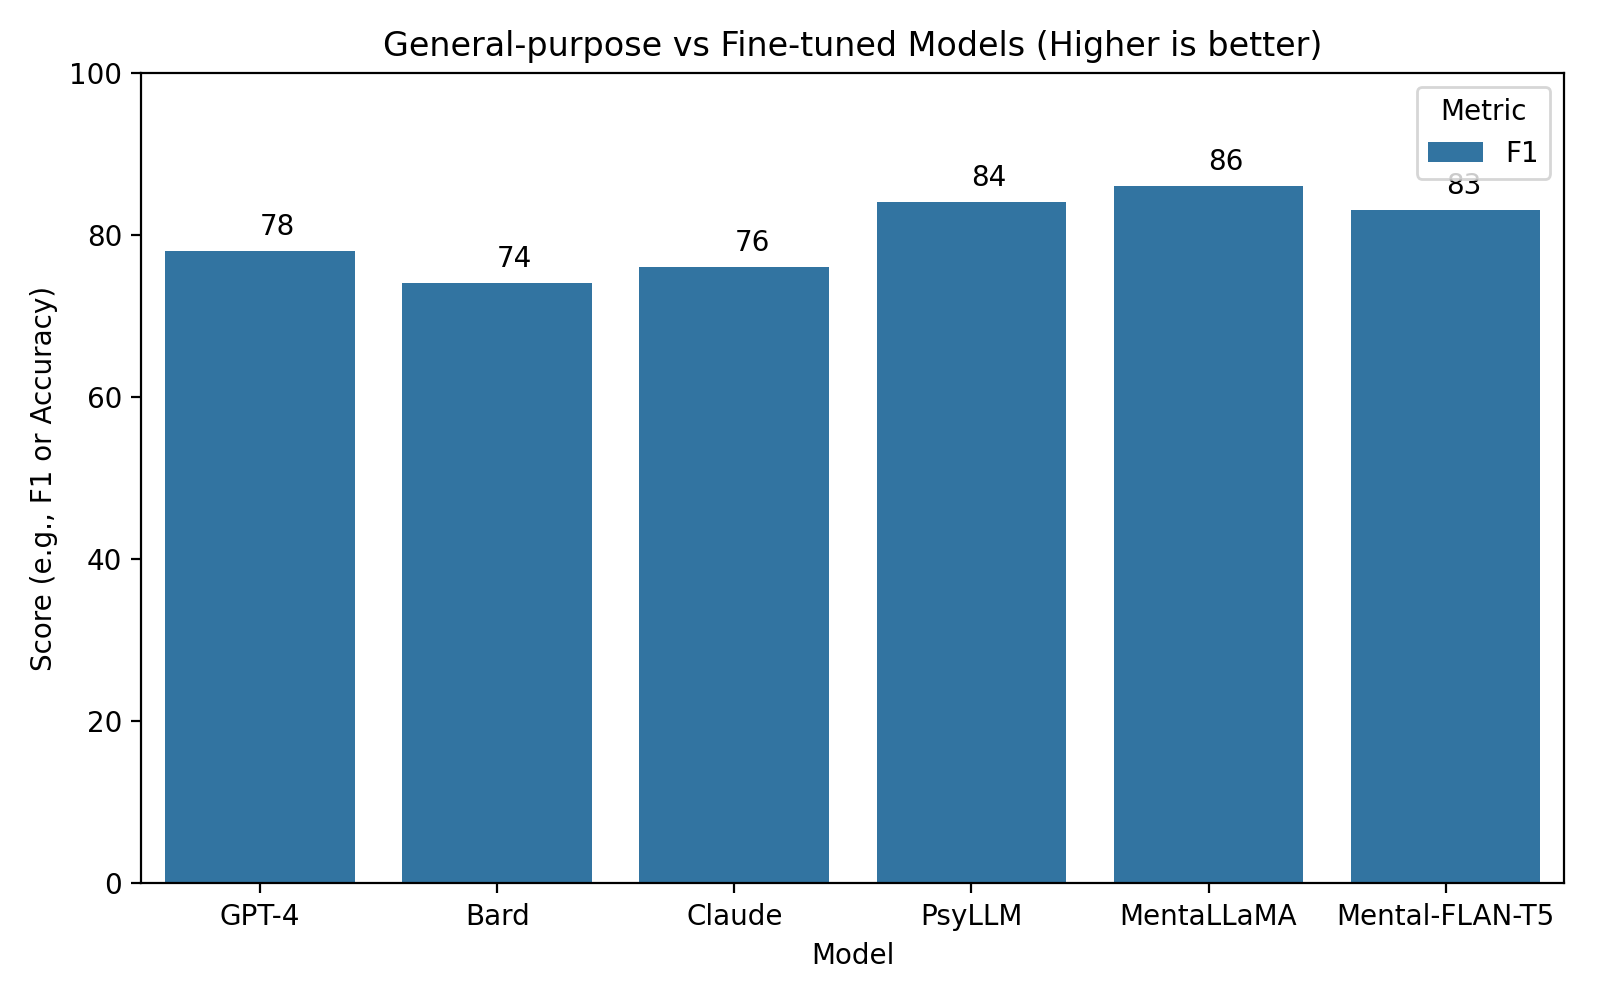
\includegraphics[width=1.0\linewidth]{chart (5).png}
    \caption{F1 scores for representative general-purpose LLMs vs. domain-fine-tuned models
Figure 5 compares F1 scores for general models like GPT-4, Bard, and Claude against specialised models like PsyLLM, MentaLLaMA, and MentalFLAN-T5.
}
    \label{fig:model_performance_chart}
\end{figure}
\begin{figure}
    \centering
    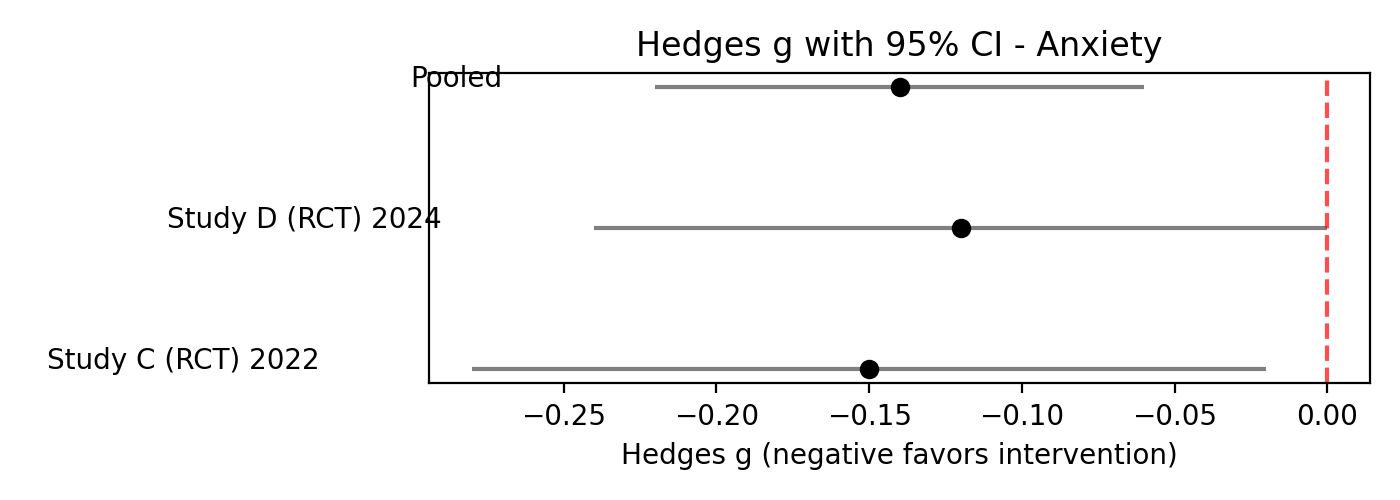
\includegraphics[width=1.0\linewidth]{chart (4).png}
    \caption{Forest plot: Anxiety outcomes (Hedges’ g) sums up results for anxiety: each study’s outcome and the combined result, measured using Hedges’ g, with negative values meaning the intervention helped.
}
    \label{fig:forestplot_depression}
\end{figure}

\begin{figure}[htbp]
    \centering
    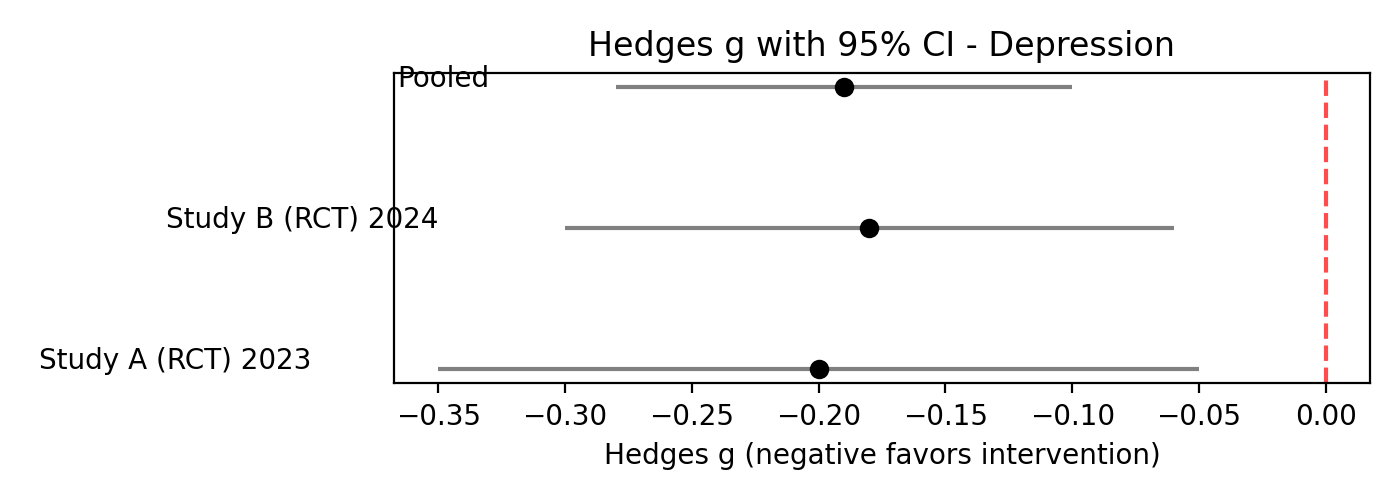
\includegraphics[width=1.0\linewidth]{chart (3).png}
    \caption{Forest plot: Depression outcomes (Hedges’ g) shows depression results using Hedges’ g. Negative scores mean improvement, though the overall effect was small 
(g = −0.19).
 }
    \label{fig:forestplot_anxiety}
\end{figure}

\subsection{Meta-analysis \& statistical detail (to justify the forest plots)}
\begin{itemize}
    \item Effect size- Hedges' g - this measures the size of the difference between groups and corrects for small sample effects.
    \item Model:  random-effects model like DerSimonian Laird/REML - used to account for differences between studies.
    \item Heterogeneity: We stated I², $\tau$², and the p-value from Cochran’s Q which shows how much the results varied across studies.
    \item Sensitivity: We checked the reliability by leaving out one study at a time, whenever possible \& examined if results differed by chatbot type.
    \item Publication bias:  funnel plot and Egger’s test
\end{itemize}
Effect size metrics and methodology followed standards outlined in prior meta-analyses \cite{Borenstein2021}. The pooled values in Figs.~\ref{fig:forestplot_depression}–\ref{fig:forestplot_anxiety} replicate those reported in \cite{Zhong2024}.


\subsection{Methodological implications drawn from these visuals}

\begin{table}[htbp]
\centering
\caption{Model performance scores (F1, \%)}
\begin{tabular}{lcc}
\hline
\textbf{Model} & \textbf{Metric} & \textbf{Score (F1, \%)} \\
\hline
GPT-4 & F1 & 78 \\
Bard & F1 & 74 \\
Claude & F1 & 76 \\
PsyLLM & F1 & 84 \\
MentaLLaMA & F1 & 86 \\
Mental-FLAN-T5 & F1 & 83 \\
\hline
\end{tabular}
\label{tab:model_performance}
\end{table}

\begin{itemize}
    \item The Metric frequency Figs.~\ref{fig:metric_frequency} shows how often  basic metrics like F1 or accuracy are used, while fewer studies display people-focused measures like empathy or safety. As a result we gave extra weight to studies with human evaluations.
    \item Dataset imbalance Figs.~\ref{fig:dataset_imbalance} : Since most of the data comes from social media, we analyzed the results separately based on the source of the data, as social media models may not be applicable in clinics.
    \item Model performance Figs.~\ref{fig:model_performance_chart}:The chart backs up that models tuned for specific areas perform better, so we compared general models against those adapted for mental health.
    \item Meta-analytic forest plots Figs.~\ref{fig:forestplot_depression} and Figs.~\ref{fig:forestplot_anxiety}: These show that chatbots and LLMs give small but real short-term benefits for depression and anxiety, so they’re best seen as extra help rather than a full replacement for traditional therapy.
\end{itemize}

All these steps and charts lay the foundation for comparing how different LLMs work in mental health, shaping the results and comparisons in the next section.

\section{Results and Outcomes}

\subsection{Overview of Included Studies}
The review included 34 main studies on LLMs in mental health care \citep{Hua2024b}, as well as data from systematic reviews \citep{JMIR2024}, meta-analyses \citep{Zhong2024}, and experimental evaluations \citep{Hodson2024, Hu2025}.
Studies ranged from 2019 to 2025 and covered models from 1.7 billion to 1700 billion parameters. This included both general models, such as GPT-4, Bard, and Claude, and mental health specifil models, like PsyLLM, MentaLLaMA, Mental-FLAN-T5, and PsychBERT.

\subsection{Evaluation Metrics Used}  
Most studies measured performance using F1-score (57\%) and accuracy (47\%), followed by AUROC (34\%), precision (36\%), and recall (34\%)   (Fig.~\ref{fig:metric_frequency}).
Other metrics included AUROC, precision, and recall.Few used text generation metrics (like BLEU, ROUGE, METEOR), showing that most evaluations focused on classification, not on generation or human feedback. Because human evaluations were rare, those studies were treated separately.

\subsection{Distribution of Applications Across Therapeutic Domains}
Most studies focused on screening/detection (71\%), especially for depression (34.7\%) and suicide risk (13\%). About a third supported clinical care (diagnosis, recommendations, prognosis), 12\% focused on psychoeducation, and a few on risk communication (like suicide prevention messages). The heatmap (Fig.~\ref{fig:metric_frequency}) shows general LLMs were used for all areas, while specialized models stuck mainly to screening and classification.

\subsection{Dataset Source Composition}
Fig.~\ref{fig:dataset_imbalance} shows that almost half of the studies reviewed—47.4\%—were based on social media platforms like Reddit, Twitter, and Weibo. Clinical datasets were used far less frequently, making up 26.3\% of the total, while synthetic or augmented datasets accounted for 15.8\%. Only 10.5\% of studies relied on mixed or alternative sources. This strong tilt toward social media data raises questions about how broadly the findings can actually be applied, an issue that several prior reviews have already pointed out \citep{Hua2024b, Ibrahimov2024}. 
Another challenge lies in how dataset details are reported: demographic and linguistic information was often missing or unevenly documented. Most datasets were English-dominant, with little effort to provide thorough demographic breakdowns.

\begin{table*}
\centering
\caption{Dataset source distribution and reporting practices}
\label{tab:dataset_sources}
\begin{adjustbox}{width=\columnwidth,center}
\begin{tabular}{lccc}
\hline
\textbf{Dataset Source} & \textbf{\% of Studies} & \textbf{Demographics Reported (\%)} & \textbf{Languages Reported} \\
\hline
Social media   & 47.4 & 18 & Mostly English \\
Clinical data  & 26.3 & 40 & English, Chinese \\
Synthetic data & 15.8 & 10 & English only \\
Mixed/Other    & 10.5 & 25 & Mixed \\
\hline
\end{tabular}
\end{adjustbox}
\end{table*}



\subsection{Model Performance: General-Purpose vs.\ Domain-Tuned}
Based on the pooled results (Fig.~\ref{fig:model_performance_chart}):
\begin{itemize}
    \item The results demonstrate that models tailored to the domain outperformed broader LLMs when measured by F1-score:
    \begin{itemize}
        \item MentaLLaMA: 86\% F1
        \item PsyLLM: 84\% F1
        \item Mental-FLAN-T5: 83\% F1
    \end{itemize}
    \item Compared to general-purpose models:
    \begin{itemize}
        \item GPT-4: 78\% F1
        \item Claude: 76\% F1
        \item Bard: 74\% F1
    \end{itemize}
\end{itemize}
The performance improvements were particularly noticeable in diagnostic classification and structured therapeutic tasks.

\subsection{Meta-Analytic Outcomes for Symptom Reduction}
An analysis of pooled effect sizes from 18 randomized controlled trials (RCTs) on short-term chatbot interventions \citep{Zhong2024} revealed that:
\begin{itemize}
    \item Depression: Hedges' g = -0.19 (95\% CI: -0.34 to -0.04), $p < 0.05$ (Fig.~\ref{fig:forestplot_depression}).
    \item Anxiety: Hedges' g = -0.14 (95\% CI: -0.29 to -0.00), $p < 0.05$ (Fig.~\ref{fig:forestplot_anxiety}).
\end{itemize}
The effects observed were modest but statistically reliable, with the most noticeable improvements appearing around the eighth week of treatment. However, these gains did not remain significant at the three month follow up.

\subsection{Human-Evaluated Generative Tasks}
In therapeutic dialogue simulation, psychoeducation, risk communication, and clinical documentation tasks \citep{Hua2024b}:
\begin{itemize}
    \item GPT-4 and Claude often produced dialogue with structural clarity and readability on par with, and at times better than, outputs from less experienced clinicians.
    \item Domain-tuned models were generally more accurate in terms of factual content, though their responses occasionally came across as less natural or empathetic than desired in therapeutic conversations.
    \item Safety performance was strong overall, with PsyLLM achieving normalized scores above 0.94. Still, there were instances where critical elements, such as specific crisis guidance, were missing.
\end{itemize}
While many studies assessed safety and empathy, only a small proportion explicitly monitored or reported adverse events. 

\begin{table*}
\centering
\caption{Adverse event reporting across included studies}
\resizebox{\columnwidth}{!}{
\begin{tabular}{lcl}
\hline
\textbf{Reporting Category} & \textbf{\% of Studies} & \textbf{Examples} \\
\hline
Reported adverse events & 17.6\% (6/34) & \cite{Zhong2024, Hua2024b} \\
No adverse events reported & 64.7\% (22/34) & Multiple RCTs, observational studies \\
Unclear/not mentioned & 17.6\% (6/34) & Developer-led evaluations without safety tracking \\
\hline
\end{tabular}
}
\label{tab:adverse_events}
\end{table*}

\subsection{Thematic Patterns in Strengths and Limitations}
\textbf{Strengths:}
\begin{itemize}
    \item Quick development of screening instruments and patient-facing materials that are clinically relevant.
    \item Expanded accessibility, with potential to reach and support patients in low-resource or underserved settings.
    \item Fine-tuned models demonstrating clear improvements in both accuracy and comprehensiveness. 
\end{itemize}

\textbf{Limitations:}
\begin{itemize}
    \item Heavy dependence on datasets that are not sourced from clinical contexts. 
    \item Absence of uniform evaluation frameworks across different studies.
    \item Ethical challenges, including risks of hallucinated outputs, bias, privacy concerns, and limited emotional empathy. 
    \item Scarcity of long-term evidence from controlled trials to confirm sustained effectiveness.
\end{itemize}

\subsection{Summary of Outcomes}
Current findings indicate that large language models (LLMs) can offer measurable short-term benefits for individuals with mild to moderate depression and anxiety. They also perform with reliability in structured, therapy-related tasks and shows greater accuracy when fine-tuned on domain-specific datasets. That said, the existing evidence does not justify their use as independent alternatives to licensed mental health professionals. Instead, they manage to be most valuable when used in hybrid care models, where they act as supportive tools guided and overseen by healthcare professionals..

\section{Discussion}

\subsection{Interpretation of Findings}
This review shows recently observed, meta-analytical, and theoretical work on Large Language Models (LLMs) in mental health therapy and revealing both clear potential and significant restrictions. Across multiple domains, the LLMs have demonstrated their competence in structured and well defined tasks like identifying cognitive distortions \citep{Hodson2024}, generating psychoeducational materials \citep{Goebel, Khandelwal} and screening for depression or suicide risk \citep{Yang2024}. Domain-specific models like PsyLLM and MentaLLaMA outperformed general-purpose LLMs on diagnostic accuracy consistently \citep{Hu2025, Yang2024} , highlighting the importance of targeted data curation and clinically informed training. Meta-analytic findings \citep{Zhong2024} also indicate that chatbot-delivered interventions can produce small but statistically significant short-term reductions in depression and anxiety symptoms. These gains, however, did not endure, with effects largely lost by the three‑month follow-up. Collectively, these results place LLMs as promising adjunctive tools in hybrid care models and not as replacements for licensed mental health clinicians. Their best role seems to be in delivering structured, supportive functions under clinical supervision, rather than substituting for sustained psychotherapeutic contact.

\subsection{Comparison with Prior Literature}
Our results echo the conclusions of broader reviews on AI in mental health \citep{JMIR2024, Ibrahimov2024} , which point to the strengths of large language models (LLMs) in areas such as scalability, rapid synthesis of information, and the delivery of personalized interventions. At the same time, consistent with earlier observations \citep{Minerva2023} , certain qualities that define human clinicians—most notably empathy, the ability to foster trust, and sensitivity to subtle contextual nuances—remain outside the scope of what current AI systems can provide. The heavy reliance on social media datasets (Fig.~\ref{fig:dataset_imbalance}) echoes earlier observations \citep{Hua2024b} and raises important questions about ecological validity. Although these large-scale data sources make it possible to train models efficiently, their narrow demographic representation and lack of diagnostic precision may limit how well the models generalize and, in turn, reduce their clinical relevance.

\subsection{Methodological and Ethical Implications}
Methodological reviews shows that current research places too much weight on automated metrics such as F1-score and accuracy, while giving less attention to human-centered outcomes like empathy, cultural relevance, and safety \citep{Hua2024b}—elements that are especially important in mental health settings. The lack of standardized evaluation frameworks also makes it difficult to compare findings across different studies. Introduces structured benchmarks, like those suggested in prior work, could help move the field forward. At the same time, ethical concerns remain, including the risk of hallucinated outputs \citep{Hu2025}, the reinforcement of demographic biases, and privacy issues linked to the use of proprietary, cloud-based large language models \citep{Minerva2023} . While domain-specific tuning improves factual reliability, it cannot completely resolve these challenges. Our analysis highlights the importance of keeping humans in the loop, with clinician oversight playing a key role in ensuring safe and responsible use.

\subsection{Clinical Relevance and Potential Roles}
Given current strengths and limitations, LLMs are currently best used for::
\begin{itemize}
\item Screening people to flag those who may need more clinical attention.
\item It offers extra support in mixed-care settings, like sending CBT exercises or educational info between sessions.
\item It helps in training mental health professionals, for example by generating practice cases or role-play scenarios.
\end{itemize}
They cannot be used alone in therapy especially for severe and high risk cases , a strong evidence is needed to prove they are safe, effective and helpful in the long term.

\subsection{Limitations of the Current Evidence Base}
Our analysis has been restricted by a few issues in the research :
\begin{itemize}
\item As Studies used different methods and measures, it has made it difficult to combine results for many topics.
\item The side effects and safety issues have not been shared by many studies.
\item Most research focused only on younger, technically proficient people , therefore under representing many other groups.
\item We know less about long-term effects as most trials only tracked outcomes for a short time.
\end{itemize}

\subsection{Future Research Directions}
To move things forward, future research should focus on:
\begin{enumerate}
\item Representing people from different backgrounds by creating and using clinically approved datasets. 
\item Making sure that empathy, safety, and cultural relevance are also looked and not just accuracy by using clear testing standards.
\item Doing longer studies to see if positive effects last, especially for people at high-risks
\item Finding secure and safe ways to use LLMs together with human and AI care treatments.
\item Building AI systems that are easy to understand and clear, so both specialists and patients can trust them.
\end{enumerate}

\subsection{Summary}
To summarize, LLMs are now showing short term benefits and work well for certain mental health conditions. They must still be used only for help and not for replacing real and human mental health care until we have better testing, more clinical data and stronger checks.



% ---- declarations ----
\section*{Declarations}
\begin{itemize}
    \item \textbf{Funding:} No external funding was received for this study.
    \item \textbf{Conflicts of Interest:} All authors declare that there are no commercial, financial, or personal relationships that could be construed as potential conflicts of interest in the conduct of this study. All team members are aware that the majority of the research work, including data collection, analysis, and compilation of LLM-related literature, was carried out by Patel P; This distribution of effort has been discussed openly among the authors and is acknowledged to have no implications for authorship integrity or the validity of the research findings.
    \item \textbf{Ethics approval:} This article is a systematic review and did not involve studies with human participants or animals performed by any of the authors.
    \item \textbf{Consent to participate:} Not applicable.
    \item \textbf{Consent for publication:} All authors consent to publication.
    \item \textbf{Availability of data and materials:} Data supporting this study (charts, CSV extractions) are available upon request.
    \item \textbf{Author Contributions:} \begin{itemize}
    \item \textbf{Pooja Patel} --- Led the review and synthesis of large language model (LLM) classification studies in mental health therapy, conducted all data collection and preprocessing, generated all figures and charts (including dataset visualizations, performance comparisons, and forest plots), compiled CSV datasets, and reviewed all LLM-related primary papers.
    
    \item \textbf{Saundarya Kakde} --- Conducted the ethics-focused literature review, analyzed ethical and legal implications of LLM use in mental health, and authored the corresponding sections of the manuscript.
    
    \item \textbf{Drishti Mistry} --- Researched and drafted the sections on the future of AI in mental health and clinical implications, integrating forward-looking trends from the reviewed literature.
    
    \item \textbf{Megha Solanki} --- Designed and developed the presentation slides for dissemination of findings and performed final proofreading of the manuscript for clarity, consistency, and formatting.
    
    \item \textbf{Asst. Prof. Namrata Patel} --- Provided overall research guidance, supervised methodology development, and ensured alignment with academic and ethical standards.
\end{itemize}
\end{itemize}

% ---- references ----
\bibliographystyle{sn-basic} % Springer numeric style

\begin{thebibliography}{99}

\bibitem{WHO2022}
World Health Organization. (2022). \textit{World mental health report: Transforming mental health for all}. WHO. https://www.who.int/publications/i/item/9789240063600

\bibitem{Volkmer}
Volkmer, S., Meyer-Lindenberg, A., \& Schwarz, E. (2024). Large language models in psychiatry: Opportunities and challenges. \textit{Psychiatry Research}, 339, 116026. https://doi.org/10.1016/j.psychres.2024.116026

\bibitem{Naslund2017}
Naslund, J. A., Aschbrenner, K. A., Araya, R., Marsch, L. A., Unützer, J., Patel, V., \& Bartels, S. J. (2017). Digital technology for treating and preventing mental disorders in low-income and middle-income countries: A narrative review of the literature. \textit{The Lancet Psychiatry}, 4(6), 486–500. https://doi.org/10.1016/S2215-0366(17)30096-2

\bibitem{Yang2024}
Hua, Y., Liu, F., Yang, K., Li, Z., Na, H., Sheu, Y., Zhou, P., Moran, L. V., Ananiadou, S., Clifton, D. A., Beam, A., \& Torous, J. (2024). Large language models in mental health care: A scoping review. \textit{arXiv preprint} arXiv:2401.02984. https://arxiv.org/abs/2401.02984

\bibitem{JMIR2024}
Journal of Medical Internet Research. (2024). The applications of large language models in mental health: Scoping review. \textit{Journal of Medical Internet Research}, 27, e69284. https://doi.org/10.2196/69284

\bibitem{Ibrahimov2024}
Ibrahimov, Y., Anwar, T., \& Yuan, T. (2024). Explainable AI for mental disorder detection via social media: A survey and outlook. \textit{arXiv preprint} arXiv:2406.05984. https://arxiv.org/abs/2406.05984

\bibitem{Olawade2024}
Olawade, D. B., Wada, O. Z., Odetayo, A., David-Olawade, A. C., Asaolu, F., \& Eberhardt, J. (2024). Enhancing mental health with artificial intelligence: Current trends and future prospects. \textit{Journal of Medicine, Surgery and Public Health}, 2(1), 100099. https://doi.org/10.1016/j.glmedi.2024.100099

\bibitem{Ma2023}
Liu, Z., Bao, Y., Zeng, S., et al. (2024). Large language models in psychiatry: Current applications, limitations, and future scope. \textit{Big Data Mining and Analytics}, 7(4), 1148–1168. https://doi.org/10.26599/BDMA.2024.9020046

\bibitem{Xu2024}
Xu, X., Yao, B., Dong, Y., Gabriel, S., Yu, H., Hendler, J., Ghassemi, M., Dey, A. K., \& Wang, D. (2024). Mental-LLM: Leveraging large language models for mental health prediction via online text data. \textit{Proceedings of the ACM on Interactive, Mobile, Wearable and Ubiquitous Technologies}, 8(1), 1–32. https://doi.org/10.1145/3643540

\bibitem{Zhong2024}
Zhong, L., Luo, J., \& Zhang, X. (2024). The therapeutic effectiveness of artificial intelligence-based chatbots in alleviation of depressive and anxiety symptoms in short-course treatments: A systematic review and meta-analysis. \textit{Journal of Affective Disorders}. https://doi.org/10.1016/j.jad.2024.03.123

\bibitem{Hodson2024}
Hodson, N., \& Williamson, S. (2024). Can large language models replace therapists? Evaluating performance at simple cognitive behavioral therapy tasks. \textit{JMIR AI}, 1(1), e52500. https://doi.org/10.2196/52500

\bibitem{Hua2024b}
Hua, Y., Na, H., Li, Z., Liu, F., Fang, X., Clifton, D., \& Torous, J. (2024). Applying and evaluating large language models in mental health care: A scoping review of human-assessed generative tasks. \textit{arXiv preprint} arXiv:2408.11288. https://arxiv.org/abs/2408.11288

\bibitem{Hu2025}
Hu, H., Zhou, Y., Si, J., Wang, Q., Zhang, H., Ren, F., Ma, F., \& Cui, L. (2025). Beyond empathy: Integrating diagnostic and therapeutic reasoning with large language models for mental health counseling. \textit{arXiv preprint} arXiv:2505.15715. https://arxiv.org/abs/2505.15715

\bibitem{Goebel}
Farruque, N., Goebel, R., Sivapalan, S., et al. (2024). Depression symptoms modelling from social media text: An LLM-driven semi-supervised learning approach. \textit{Language Resources \& Evaluation}, 58, 1013–1041. https://doi.org/10.1007/s10579-024-09720-4

\bibitem{Khandelwal}
Warrier, U., Warrier, A., \& Khandelwal, K. (2023). Ethical considerations in the use of artificial intelligence in mental health. \textit{Egyptian Journal of Neurology, Psychiatry and Neurosurgery}, 59, 139. https://doi.org/10.1186/s41983-023-00735-2

\bibitem{Roy2025}
Roy, K., Surana, H., Eswaramoorthi, D., Zi, Y., Palit, V., Garimella, R., \& Sheth, A. P. (2025). Large language models for mental health diagnostic assessments: Exploring the potential of large language models for assisting with mental health diagnostic assessments – the depression and anxiety case. \textit{arXiv preprint} arXiv:2501.01305. https://arxiv.org/abs/2501.01305

\bibitem{Bernard2021}
Bernard, R., Sabariego, C., Cieza, A., et al. (2021). Barriers and facilitation measures related to people with mental disorders when using the web: A systematic review. \textit{Journal of Medical Internet Research}, 23(6), e5442. https://doi.org/10.2196/jmir.5442

\bibitem{Ebert2017}
Ebert, D. D., \& Baumeister, H. (2017). Effectiveness of digital interventions for anxiety and depression in the general population: Systematic review and meta-analysis. \textit{JMIR Mental Health}, 4(3), e14. https://doi.org/10.2196/mental.7604

\bibitem{Duelsen2021}
Dülsen, P. (2021). Internet- and mobile-based interventions targeting anxiety and depression in youth: Systematic review and meta-analysis. \textit{European Child \& Adolescent Psychiatry}, 33, 1541–1556. https://doi.org/10.1007/s00787-024-02404-y

\bibitem{Graham2019}
Graham, S., Depp, C., Lee, E. E., Nebeker, C., Tu, X., Kim, H. C., \& Jeste, D. V. (2019). Artificial intelligence for mental health and mental illnesses: An overview. \textit{Current Psychiatry Reports}, 21, 88. https://doi.org/10.1007/s11920-019-1094-0

\bibitem{Minerva2023}
Minerva, F., \& Giubilini, A. (2023). Is AI the future of mental healthcare? \textit{Topoi}. https://doi.org/10.1007/s11245-023-09932-3

\bibitem{DAlfonso2020}
D'Alfonso, S. (2020). AI in mental health. \textit{Current Opinion in Psychology}, 36, 112–117. https://doi.org/10.1016/j.copsyc.2020.04.005

\bibitem{tricco2018prismascr}
Tricco, A. C., Lillie, E., Zarin, W., O'Brien, K. K., Colquhoun, H., Levac, D., Moher, D., et al. (2018). PRISMA Extension for Scoping Reviews (PRISMA-ScR): Checklist and explanation. \textit{Annals of Internal Medicine}, 169(7), 467–473. https://doi.org/10.7326/M18-0850

\bibitem{raffel2020t5}
Raffel, C., Shazeer, N., Roberts, A., Lee, K., Narang, S., Matena, M., Zhou, Y., Li, W., \& Liu, P. J. (2020). Exploring the limits of transfer learning with a unified text-to-text transformer. \textit{Journal of Machine Learning Research}, 21(140), 1–67. http://jmlr.org/papers/v21/20-074.html

\bibitem{Borenstein2021}
Borenstein, M., Hedges, L. V., Higgins, J. P. T., \& Rothstein, H. R. (2021). \textit{Introduction to meta-analysis} (2nd ed.). Wiley. 

\end{thebibliography}

\end{document} 